\documentclass[border=10pt]{standalone}

\usepackage{tikz}
\usepackage{tikzsymbols}
\usetikzlibrary{calc,patterns,shapes.geometric}

\def\centerarc[#1](#2)(#3:#4:#5){\draw[#1] ($(#2)+({#5*cos(#3)},{#5*sin(#3)})$) arc (#3:#4:#5);}

\begin{document}
	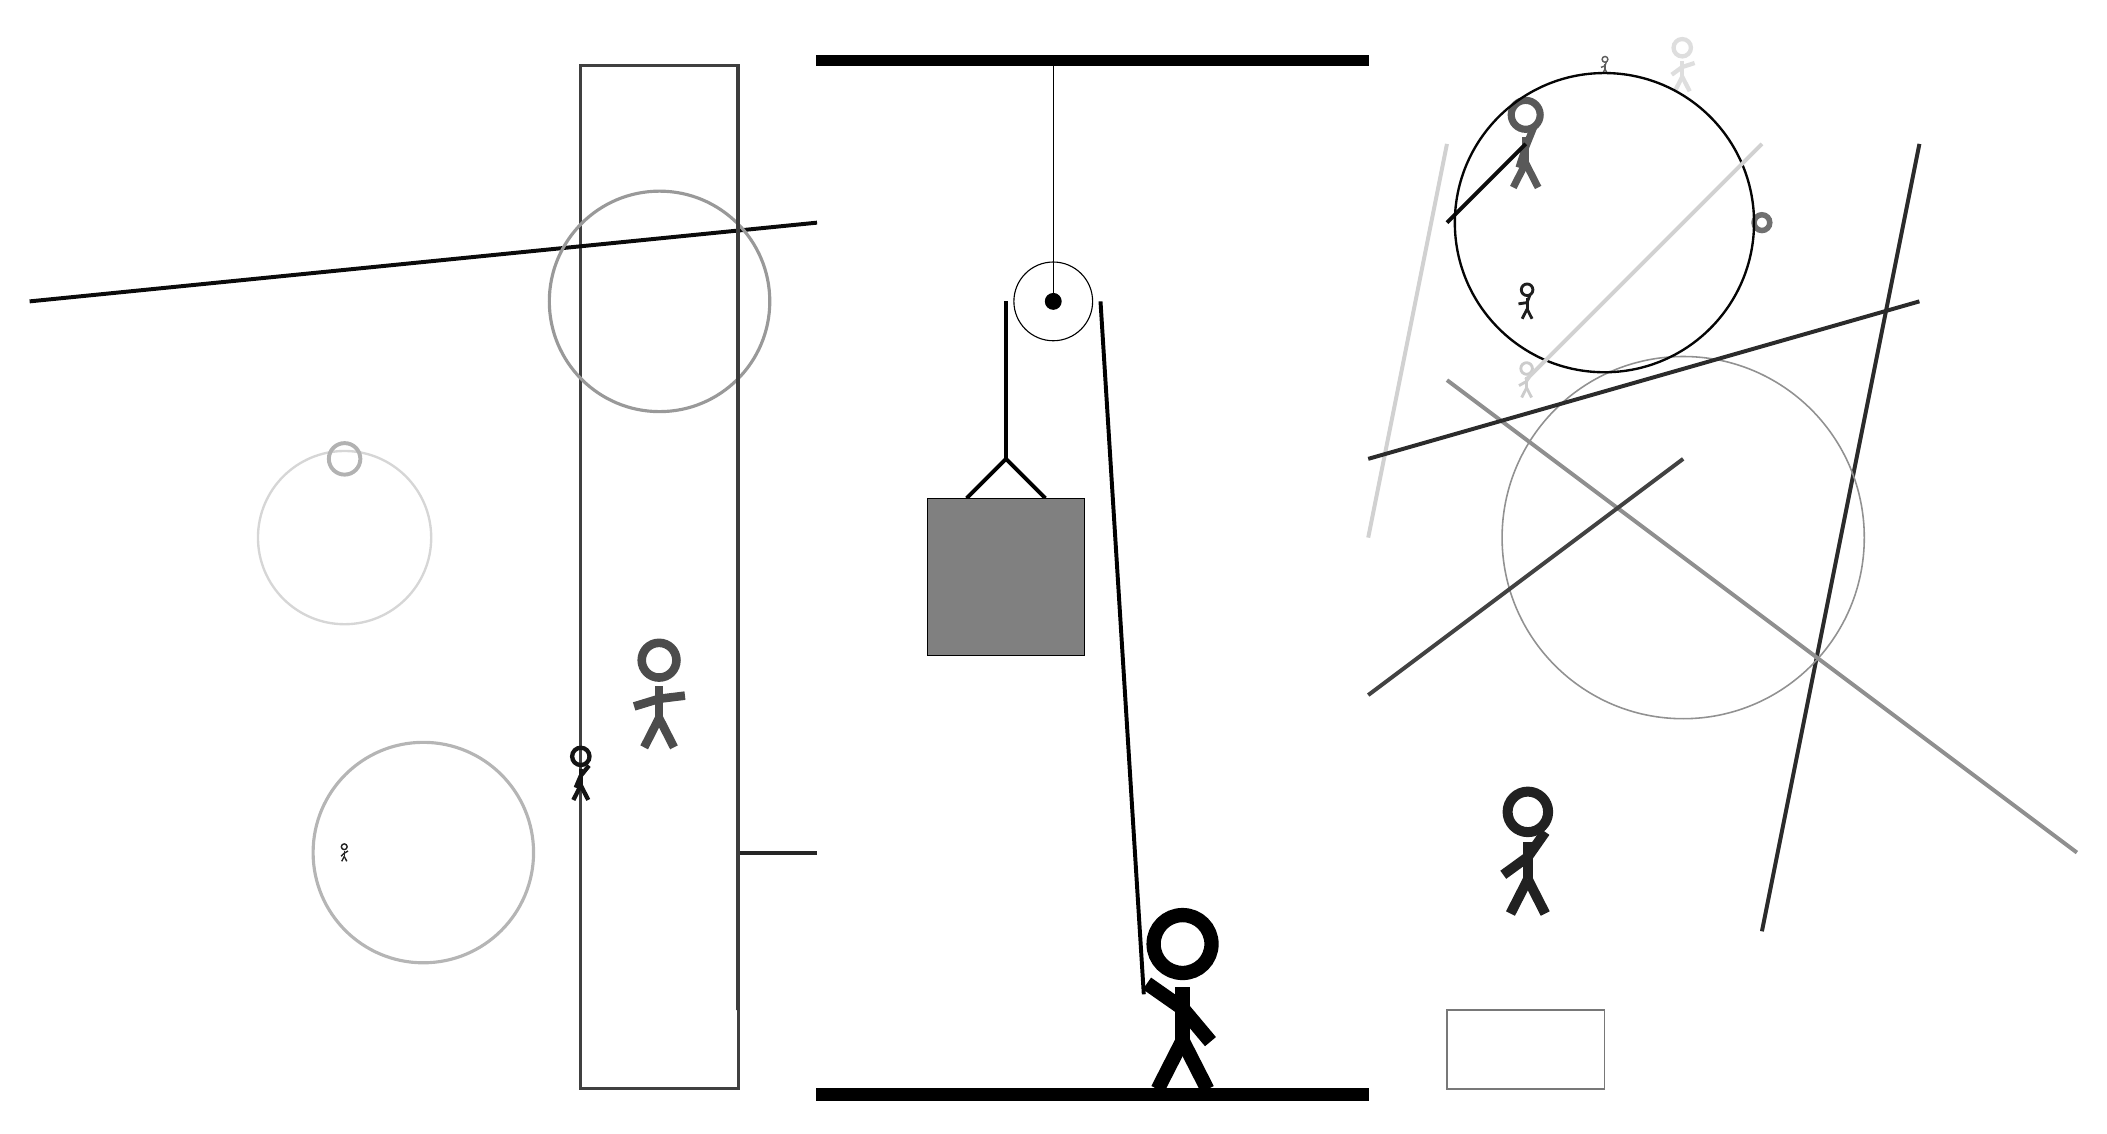
\begin{tikzpicture}
		%%%%% START %%%%%
		
		\draw[fill=black] (-2, 10) rectangle (5, 10.125);
		
		\draw[line width=0.5mm, color=black!83](10, -1) -- (12, 9);
		
		\draw [line width=0.3mm, color=black!16](-8, 4) circle (1.1);
		\draw[line width=0.4mm, color=black!75] (-3, 10) rectangle (-5, -3);
		\node[line width=0.5mm, color=black!20] at (7, 6) {\Strichmaxerl[2][29][57]};
		\draw[line width=0.5mm, color=black!96](-2, 8) -- (-12, 7);
		\node[line width=0.2mm, color=black!13] at (9, 10) {\Strichmaxerl[3][36][18]};
		\draw [line width=0.5mm, color=black!30](-8, 5) circle (0.2);
		\draw[line width=0.2mm, color=black!53] (6, -2) rectangle (8, -3);
		\draw[line width=0.5mm, color=black!85](-3, 0) -- (-2, 0);
		\node[line width=0.3mm, color=black!92] at (-5, 1) {\Strichmaxerl[3][67][51]};
		\node[line width=0.4mm, color=black!65] at (7, 9) {\Strichmaxerl[5][72][68]};
		
		\draw [line width=0.2mm, color=black!43](9, 4) circle (2.3);
		\draw [line width=0.4mm, color=black!40](-4, 7) circle (1.4);
		\node[line width=0.6mm, color=black!87] at (7, 0) {\Strichmaxerl[7][36][55]};
		\node[line width=0.6mm, color=black!63] at (8, 10) {\Strichmaxerl[1][22][71]};
		\draw[line width=0.5mm, color=black!95](7, 9) -- (6, 8);
		
		\draw[line width=0.5mm, color=black!76] (-3, 10) rectangle (-3, -2);
		\draw [line width=0.4mm, color=black!29](-7, 0) circle (1.4);
		\node[line width=0.6mm, color=black!88] at (7, 7) {\Strichmaxerl[2][8][70]};
		\draw [line width=0.7mm, color=black!56](10, 8) circle (0.1);
		\draw[line width=0.5mm, color=black!44](6, 6) -- (14, 0);
		\draw[line width=0.5mm, color=black!18](5, 4) -- (6, 9);
		\draw[line width=0.5mm, color=black!83](5, 5) -- (12, 7);
		\node[line width=0.4mm, color=black!86] at (-8, 0) {\Strichmaxerl[1][45][30]};
		\node[line width=0.2mm, color=black!70] at (-4, 2) {\Strichmaxerl[6][17][7]};
		
		\draw[line width=0.5mm, color=black!74](5, 2) -- (9, 5);
		\draw [line width=0.3mm, color=black!98](8, 8) circle (1.9);
		\draw[line width=0.5mm, color=black!18](10, 9) -- (7, 6);
		
		\draw (1, 7) circle (0.5);
		\draw[fill=black] (1, 7) circle (0.1);
		\draw (1, 10) -- (1, 7);
		
		\draw[line width=0.5mm] (-0.1, 4.5) -- (0.4, 5.0) -- (0.9, 4.5);
		\draw[fill=black!50] (-0.6, 4.5) rectangle (1.4, 2.5);
		
		\draw[line width=0.5mm] (0.4, 7) -- (0.4, 5.0);
		\centerarc[line width=0.5mm](1, 7)(0:180:0.6);
		\draw[line width=0.5mm](1.6, 7) -- (2.15, -1.8);
		
		\node at (2.6, -1.9) {\Strichmaxerl[10][-35][-50]};
		
		\draw[fill=black] (-2, -3) rectangle (5, -3.15);
		
		%%%%% END %%%%%
	\end{tikzpicture}
\end{document}